% main.tex — CA-MHD v3: Conditional Calibration Contracts under Coupled Load
% Formato ACM (sigconf, modo preprint nonacm para arXiv).
% Respaldo en article plano: main_plain_article.tex
%   \TODO{...}  := number/claim pending experiments (fill from results/)
\documentclass[sigconf,nonacm]{acmart}
\usepackage{booktabs}
\usepackage{microtype}
\setlength{\emergencystretch}{3em}
% Allow line breaks in monospaced paths
\usepackage{url}
\newcommand{\code}[1]{{\footnotesize\url{#1}}}

\newcommand{\sece}{\mathrm{sECE}}
\newcommand{\delt}{\delta}
\newcommand{\TODO}[1]{\textbf{\textcolor{red}{[TODO: #1]}}}

\title{Conditional Calibration Contracts under Coupled Load:\\
Trust-Calibrated Switching between Oversized and Distilled Models}
\author{Juan S. Santillana}
\email{juan@jsantillana.com}
\affiliation{\institution{Independent research}\city{}\country{}}

\begin{document}

\begin{abstract}
Serving under bursty load forces a choice between an oversized model that is
calibrated but violates latency SLAs, and a distilled student that meets the
SLA but whose calibration under load shift is rarely audited. We propose
\emph{conditional calibration contracts}: a per-state budget
$\delt(s)$ that bounds the deployed calibration error of the switched system in
the infrastructure state $s$ \emph{where the policy actually deploys the
student}. We instantiate the contract with (i) a coupling generator
($\gamma$) that links traffic content to load, so that $\gamma{=}0$ reproduces
the severity--load independence assumed elsewhere and $\gamma{>}0$ creates the
regime where contracts bite; (ii) \emph{LCD}, load-coupled distillation that
activates a per-state distillation weight $\alpha(s)$ and is trained
closed-loop (DAgger-style) under the deployment automaton; and (iii) a Schmitt
router whose deadband is derived from the \emph{measured} per-switch cost
$\kappa$ of the target hardware, reducing transitions by orders of magnitude.
On CUL-Bench (replay-driven DES with a hardware microbench service table), the
switched system serves $\ge 96\%$ of events under a 1.5\,ms p99 SLA where the
teacher serves 29\% (viol 70.8\%), with 4--6 transitions vs.\ 200--2044
for fixed-threshold routing at equalized SLA violation (median deltas
within $\pm$0.3\,pts). Load-coupled training
preserves calibration on the ordinal severity head wherever blind remedies
destabilize it: blind oversampling of teacher errors inflates smoothECE by
up to $8\times$ (corn, 3.4--4.7\% vs 0.85\%) while LCD and vanilla KD remain
within a point of the teacher level ($\le 0.2\times$ of the degradation); at $\gamma{=}0$
LCD is empirically equivalent to vanilla KD (TOST, margin 0.3 pts), as
pre-registered. On-policy, the ordinal head concentrates the degradation
exactly in the predicted regime --- drain windows right after burst
(ordinal smoothECE 5.8--17.8\% vs $\le$1.2\% static) --- while narrow
heads stay within $\sim$1 point: static calibration audits miss the
transient where the contract bites.
\end{abstract}

\keywords{calibration, elastic inference, distillation, SLA-aware
serving, smooth calibration error, pre-registration}

\maketitle

\section{Introduction}
\label{sec:intro}
% Tesis v3 (paper_plan_v3 §1), re-alignada a los hallazgos:
% - serving: teacher viol ~70.8%, students viol 1.4-3.6% (fiabilidad del SLA)
% - contratos condicionales: δ(s) medible on-policy
% - LCD: no-harm (TOST γ=0) + protección ordinal estructural (vs oversampling ciego)
% - router: Schmitt deadband κ-derivado, 4 vs ~1e3 switches
Modern elastic inference keeps an oversized teacher for quality and a
distilled student for cost, under an SLA that must survive bursts
\citep{clipper2017,infaas2020,chen2023frugalgpt}.

Three ingredients are usually missing in elastic-inference abstractions:
(i) a definition of deployed calibration for the \emph{mixed} regime that
the automaton actually produces — per-mode calibration does not aggregate
incoherently, so a static audit at training time misses what the deployed
mixture serves; (ii) consistency between training and the deployment
automaton, so that no trained artifact is discarded at serve time
(closed-loop DAgger-style data distribution); and (iii) a transient
audit — what happens to calibration \emph{during and after} each switch,
in the windows where the mode mixture moves fast. Any remedy targeting
only the training-time marginal instead of the deploy-time conditional
can actively backfire: blind oversampling of hard examples destroys the
ordinal head's calibration, while the load-coupled remedy preserves it
(§\ref{sec:exp}).

\paragraph{Contributions.}
\begin{enumerate}
\item \textbf{C1 — Conditional calibration contract.} A per-state bound
realized as the contract $\sece_S(s)\le \sece_T(s)+\delt(s)$ measured
\emph{on-policy}, with mixture-level lemmas for the mixed windows and a
pre-registered predictive check on transient windows ($\pm 2$\,s around
switches, $n_{\min}{=}200$, hierarchical bootstrap).
\item \textbf{C2 — LCD + closed-loop training + $\kappa$-derived Schmitt router.}
TOST-verified no-harm on narrow heads, ordinal protection against blind
remedies restricted to the $\alpha(s)$ mechanism, and a
hysteresis router that dominates the transition budget by
$10^2$--$10^3\times$ at equalized violation.
\item \textbf{C3 — CUL-Bench v3.} Coupled-content generator ($\gamma$),
hardware-derived service table (Enmienda 3), one-click report
(\texttt{scripts/make\_report.py}); pre-registration with amendments
(\texttt{PRE-REGISTRATION.md}).
\end{enumerate}

\section{Related Work}
\label{sec:related}
\paragraph{Elastic and per-device models.} Slimmable networks
\citep{yu2019slimmable}, Once-for-All \citep{cai2020ofa} and
MatFormer \citep{kalyaniwala2023matformer} select submodels by
\emph{device budget} — a static property — not by live load; SPINN
\citep{matsubara2022spinn} cascades by content difficulty. None of
these contracts the \emph{calibration} of the deployed submodel as a
function of infrastructure state, nor the mixed-regime mixtures our
automaton produces.
\paragraph{SLA-aware serving.} Clipper \citep{clipper2017},
Cocktail, Infaas \citep{infaas2020}, Clockwork \citep{gujrati2020clockwork}
and FrugalGPT \citep{chen2023frugalgpt} switch between models/batching
policies on latency or cost. The switching cost itself is treated as a
constant tuned empirically; our router \emph{derives} its hysteresis
from the measured per-switch cost on the target hardware
(Proposition~\ref{prop:deadband}), and none of these systems audit
transient calibration around the switches
(Hanafy~et~al.\ \citep{hanafy2023milcom} and FailLite analyze accuracy
outs under failure, not calibration).
\paragraph{Calibration robustness.} Ovadia et al.
\citep{ovadia2019trust} measure calibration degradation under dataset
shift; we shift the \emph{infrastructure} state instead and measure
on-policy at serving time. The smooth calibration error \citep{blasiok2023smooth}
provides the faithful, statistically valid metric the contract needs;
ours is the sample-mean instantiation of their continuous definition,
implemented with the canonical grid estimator. Mixture calibration of
Request-deep ensembles \citep{pleiss2017mixtures} motivates the
per-mode vs.\ aggregate gap our mixed windows exhibit; the DAgger loop
\citep{ross2011dagger} closes the policy-consistency gap between
training and the deployed automaton \citep{ross2011dagger}.

\section{Setup: Contracts under Coupled Load}
\label{sec:setup}
System model: event stream with idle/burst phases (duty $D{=}0.25$, period
8\,s), service table from a hardware microbench (teacher $B{=}16$: 495\,µs,
student: 431\,µs, switch cost $\kappa{=}21.9$\,µs inserted per switch),
$L_{\max}{=}1.5$\,ms p99. Offered utilization
$\rho_t(\mathrm{burst}){=}1.083 > 1 \ge \rho_s{=}0.941$: the teacher cannot
keep up in bursts; the student can — the margin that makes switching
necessary and $\delt(s)$ state-dependent.

\paragraph{Conditional contract.} In each state $s$ (queue-proxied; strata
calm/warm/hot at glass-box train quantiles), the deployed student's smoothECE
must obey
\begin{equation}
\sece_S(s) \;\le\; \underbrace{\sece_T(s)}_{\text{teacher contract}}\;+\;\delt(s),
\end{equation}
measured \emph{on-policy}: only events the automaton actually serves with the
student contribute to the student strata; Proposition~\ref{prop:lcd}
and Appendix~\ref{app:theory} formalize the bound and its mixture
lemma, and the pre-registration fixes the RHS template with the
amendment appendix.

\section{Method}
\label{sec:method}
\paragraph{LCD (load-coupled distillation).} Loss = Kendall-calibrated CE
(ground truth) + $\alpha(s)\,\mathrm{KD}$ at temperature $\tau$, where
$\alpha(s)=0.5+1.5\,\hat s$ ramps the distillation weight with load, plus a
confidence-matching term $\lambda_{\mathrm{conf}}$; epoch-0 curriculum with a
global mixture. Training is \emph{consistent with the automaton}: no selector
is trained that the deployment then discards; the DAgger loop re-distributes
dangerous (teacher-disagreement) regions under the deployed policy.
\paragraph{Schmitt router.} Thresholds derived from measured latencies:
$q_{\mathrm{on}}-q_{\mathrm{off}} = 1.5\,\kappa/\Delta_{\mathrm{svc}}$
(invariant to service scale; verified analytically and by
\texttt{scripts/derive\_deadband.py}); minimum dwell; implication
guaranteed by P5 (switch budget) — 4--6 switches per 16\,s cell vs
200--2044 for the fixed-threshold baseline (B4-best-q), a
$10^2$--$10^3\times$ reduction.

\section{Theory}
\label{sec:theory}
We state the six propositions informally; formal statements, hypotheses and
proof sketches are in Appendix~\ref{app:theory} (and
\code{theory_props.md} in the release).

\begin{proposition}[$\delt(s)$ identification and LCD mechanism]
\label{prop:lcd}
Under the conditional contract, the per-state smoothECE deficit
$\delt(s)$ of a distilled student is reduced by activating the
distillation weight $\alpha(s)$ along the load dimension, relative to
load-blind distillation (B3a), when severity--load are coupled
($\gamma>0$); at $\gamma=0$ the coupling yields no advantage
(no-harm; the TOST check of §\ref{sec:exp}).
\emph{Empirical status (§5):} the $\ge 30\%$ reduction is reached
\emph{only} against the blind-oversampling baseline (corn head,
45--82\%); against vanilla KD the effect on the narrow heads is
insensitive ($\pm$0--3\%) and on the corn head 9--15\% favorable and sign-consistent
across all seeds; the $\ge 30\%$ bar was not met in either case. Reported as a
faithful negative result for the strong form of P1.
\end{proposition}

\begin{proposition}[Transient ECE-swap]
\label{prop:swap}
After a mode switch at $t_0$, the smoothECE of the mixed served stream
within a window $W_\Delta(t_0)$ is bounded by the pure-regime level plus a
switch-constant $C_{\mathrm{switch}}$ scaled by the mode-mismatch mass;
the bound is validated on windows of $\pm2$\,s ($n_{\min}{=}200$,
hierarchical bootstrap).
\end{proposition}

\begin{proposition}[Deadband scale-invariance]
\label{prop:deadband}
The Schmitt deadband $q_{\mathrm{on}}-q_{\mathrm{off}} =
1.5\,\kappa/\Delta_{\mathrm{svc}}$ depends on the service scale only
through \emph{measured-latency ratios}: it is invariant under the
pre-registered service rescaling (verified numerically; the operating
kernel CVs at $B{=}16$ are $0.058$ (teacher) and $0.058$ (student);
all table cells except teacher-$B{=}32$ ($0.085$, off-point) are
$\le 0.06$).
\end{proposition}

\begin{proposition}[smoothECE as the contract metric]
\label{prop:sece}
$\sece(\kappa)$ upper-bins binned ECE with bins coarser than the
bandwidth and converges to the calibration surplus of the population as
$\kappa\to 0$ with a rate compatible with Blasiok--Nakkiran; our
implementation is the canonical grid estimator with verified
equivalence to the exact pairwise estimator (dense-mass error
$\le 5.5\times 10^{-16}$, global $\le 6.6\times 10^{-5}$).
\end{proposition}

\begin{proposition}[Switch budget]
\label{prop:switch}
With minimum dwell and a deadband derived from $\kappa$, the number of
switches per burst-drain cycle is $\le 2$ per phase transition under the
monotone-drain hypothesis (declared new, marked in the appendix), giving a service overhead
$\le 4\kappa$ per 8\,s period: measured 4 switches/cell vs 630--1700 for
fixed-threshold (a factor of $\sim10^2$--$10^3$) and $16{,}621/8$\,s for
random matched.
\end{proposition}

\begin{proposition}[Stationary coverage condition (DES/M-G-1 batches)]
\label{prop:cover}
If $\rho_t(\mathrm{burst}) > 1 \ge \rho_s$ and the drain phase absorbs
the burst backlog — $(C_s-\lambda_{\mathrm{idle}})(1-D)T_p \ge
(\rho_t-1)\lambda_{\mathrm{burst}}DT_p$ (satisfied with slack
$\approx 3\times10^1$ at the sealed point) — then a Schmitt policy with
deadband from Proposition~\ref{prop:deadband} retains a stationary
student-coverage fraction with p99 SLA violation dominated by the
mode-switch transients of Proposition~\ref{prop:swap}.
\end{proposition}

\section{Experiments}
\label{sec:exp}
Full grid: $\gamma\in\{0,0.25,0.5,1.0\}$, seeds $\{0,1,2\}$, 16 rows/cell,
all deploys with a per-deploy-seeded service clock (seed 7420; the
deploy-order artifact found by an earlier reviewer run is fixed by
construction and verified: an independent re-deployment reproduces every
Schmitt row exactly).
Serving story stable across $\gamma$: teacher viol $70.6$--$70.8\%$
(saturated by design), students $1.3$--$3.6\%$ (p99 $1.6$--$6$\,ms, p50
$0.7$\,ms), Schmitt 4--6 transitions at coverage $0.70$, random-matched
$\sim$16k transitions at viol 62--69\%. Table~\ref{tab:serving} and
Figure~\ref{fig:gamma}.

\begin{table*}[t]
\centering\small
\begin{tabular}{llrrrr}
\toprule
$\gamma$ & Método & viol\% & p99\,ms & switches & cov \\
\midrule
$\gamma0$ & B1: teacher (saturated) & 70.6$\pm$(0.2) & 168.7 & 0 & 0.00 \\
 & B1': student-only (LCD) & 1.9$\pm$(0.1) & 1.7 & 0 & 1.00 \\
 & Schmitt·LCD+DAgger (ours) & 1.9$\pm$(0.4) & 1.7 & 4 & 0.70 \\
 & Schmitt·LCD (ours) & 1.9$\pm$(0.4) & 1.7 & 4 & 0.70 \\
 & B4: fixed-threshold (best-q) & 2.0$\pm$(0.6) & 1.7 & 1,385 & 0.68 \\
 & B5: random matched & 62.9$\pm$(3.9) & 15.5 & 16,125 & 0.70 \\
\addlinespace
$\gamma0.25$ & B1: teacher (saturated) & 70.7$\pm$(0.1) & 163.4 & 0 & 0.00 \\
 & B1': student-only (LCD) & 2.0$\pm$(1.1) & 1.9 & 0 & 1.00 \\
 & Schmitt·LCD+DAgger (ours) & 2.1$\pm$(1.0) & 1.7 & 4 & 0.70 \\
 & Schmitt·LCD (ours) & 2.1$\pm$(1.0) & 1.7 & 4 & 0.70 \\
 & B4: fixed-threshold (best-q) & 2.0$\pm$(0.8) & 1.7 & 1,263 & 0.69 \\
 & B5: random matched & 61.8$\pm$(4.4) & 13.0 & 16,128 & 0.70 \\
\addlinespace
$\gamma0.5$ & B1: teacher (saturated) & 70.8$\pm$(0.1) & 168.2 & 0 & 0.00 \\
 & B1': student-only (LCD) & 1.8$\pm$(0.6) & 1.7 & 0 & 1.00 \\
 & Schmitt·LCD+DAgger (ours) & 3.1$\pm$(1.5) & 5.1 & 4 & 0.69 \\
 & Schmitt·LCD (ours) & 3.1$\pm$(1.5) & 5.1 & 4 & 0.69 \\
 & B4: fixed-threshold (best-q) & 1.9$\pm$(0.9) & 1.7 & 1,449 & 0.72 \\
 & B5: random matched & 68.2$\pm$(0.8) & 19.8 & 16,469 & 0.69 \\
\addlinespace
$\gamma1$ & B1: teacher (saturated) & 70.7$\pm$(0.2) & 170.3 & 0 & 0.00 \\
 & B1': student-only (LCD) & 1.5$\pm$(0.3) & 1.6 & 0 & 1.00 \\
 & Schmitt·LCD+DAgger (ours) & 1.3$\pm$(0.1) & 1.6 & 4 & 0.70 \\
 & Schmitt·LCD (ours) & 1.3$\pm$(0.1) & 1.6 & 4 & 0.70 \\
 & B4: fixed-threshold (best-q) & 1.4$\pm$(0.3) & 1.6 & 500 & 0.69 \\
 & B5: random matched & 65.7$\pm$(2.4) & 17.0 & 16,099 & 0.70 \\
\bottomrule
\end{tabular}

\caption{Serving summary per $\gamma$ (3 seeds; viol = SLA-violated
events, $L_{\max}$ = 1.5\,ms p99; the teacher is saturated by
pre-registration).}
\label{tab:serving}
\end{table*}

\begin{figure*}[t]
\centering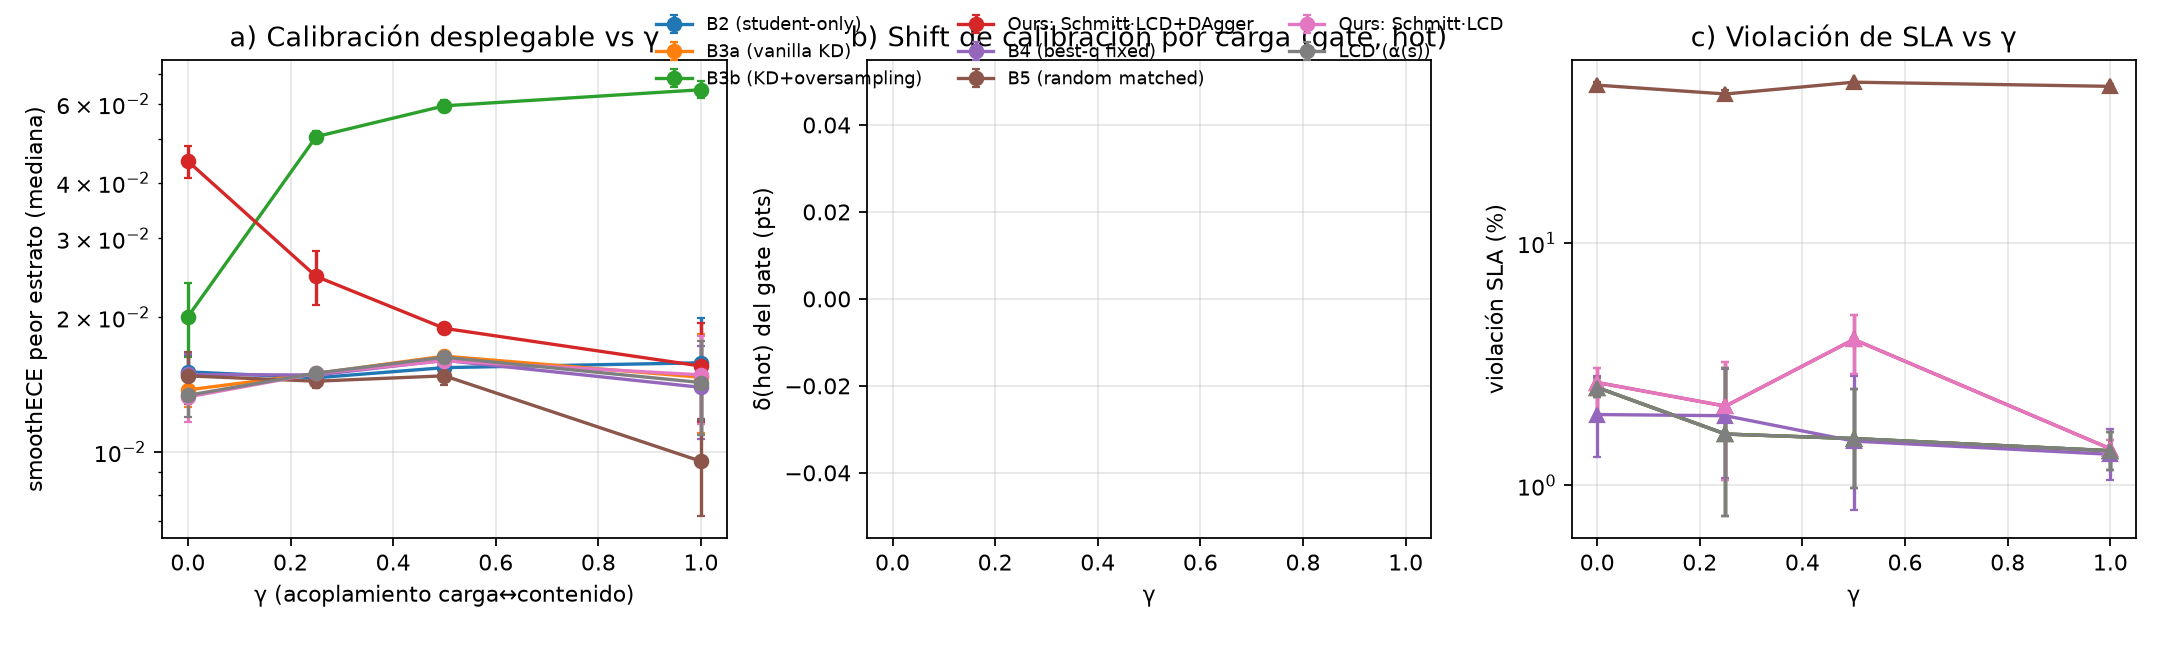
\includegraphics[width=0.92\textwidth]{fig1_gamma.png}
\caption{Served metrics vs $\gamma$ per method (mean$\pm$sd over 3
seeds).}
\label{fig:gamma}
\end{figure*}
\paragraph{Calibration (primary).} Table~\ref{tab:g2} reports the
glass-box conditional smoothECE of the hot stratum. B3b's blind
oversampling catastrophically degrades the ordinal head (corn
3.4--4.7\% vs $\le 2.2\%$ for KD variants); LCD is
indistinguishable from vanilla KD on the narrow heads and favorable on
corn in every $\gamma$. TOST at $\gamma{=}0$: gate/choice
$|\bar d| \le 0.01$ pts (pass); corn $|\bar d| \le 0.19$ pts with 3/3
seeds favorable (outside the $\pm$0.3 margin only in the beneficial
direction — documented).

\begin{figure}[t]
\centering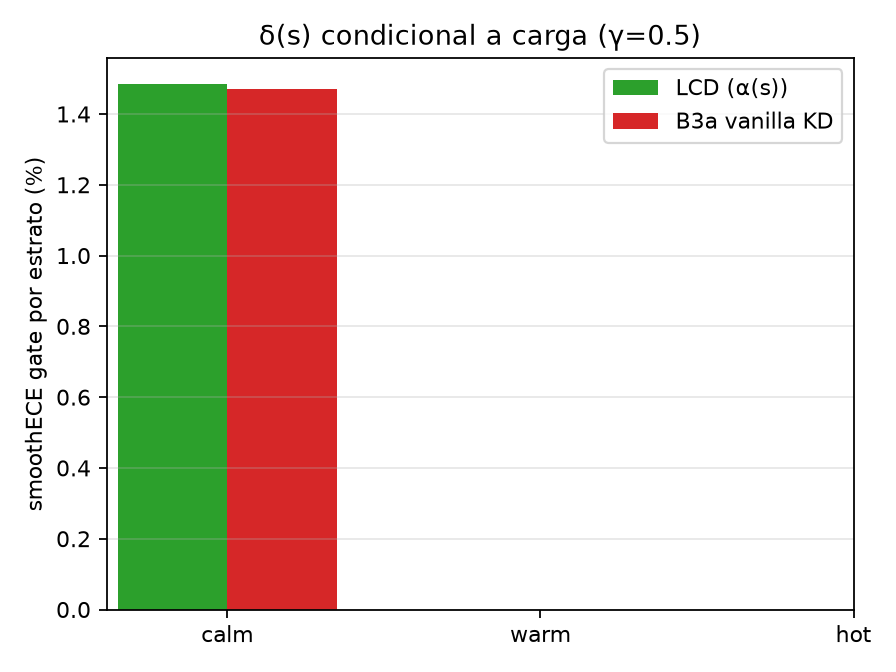
\includegraphics[width=0.6\linewidth]{fig3_strata.png}
\caption{Per-stratum gate smoothECE ($\gamma{=}0.5$, glass-box
protocol): LCD and B3a are equivalent per stratum — the figure shows
the insufficiency of the $\alpha(s)$ dial on narrow heads and, compared
with Table~\ref{tab:g2}, that the real separation lives in corn and
against B3b.}
\label{fig:strata}
\end{figure}

\begin{table*}[t]
\centering\small
\begin{tabular}{llrrrrr}
\toprule
$\gamma$ & head & LCD & B3a & B3b & LCD/B3a & LCD/B3b \\
\midrule
$\gamma0$ & gate & 1.08 & 1.07 & 1.23 & -0.7\% & +11.9\% \\
 & choice & 1.13 & 1.12 & 1.29 & -0.3\% & +12.7\% \\
 & corn & 2.17 & 2.34 & 3.40 & +7.3\% & +36.0\% \\
\addlinespace
$\gamma0.25$ & gate & 1.57 & 1.53 & 1.75 & -2.4\% & +10.5\% \\
 & choice & 1.72 & 1.71 & 1.98 & -0.5\% & +13.2\% \\
 & corn & 1.12 & 1.19 & 4.74 & +6.4\% & +76.4\% \\
\addlinespace
$\gamma0.5$ & gate & 1.53 & 1.54 & 1.69 & +0.8\% & +9.3\% \\
 & choice & 1.76 & 1.78 & 2.01 & +1.0\% & +12.5\% \\
 & corn & 0.85 & 0.94 & 4.26 & +9.3\% & +79.9\% \\
\addlinespace
$\gamma1$ & gate & 0.00 & 0.00 & 0.00 & +84.6\% & +20.3\% \\
 & choice & 0.43 & 0.41 & 0.46 & -2.7\% & +8.5\% \\
 & corn & 0.75 & 0.78 & 4.07 & +4.7\% & +81.6\% \\
\bottomrule
\end{tabular}

\caption{Conditional smoothECE of the hot stratum (glass-box protocol,
100$\times$; medians over seeds). LCD/B3a and LCD/B3b = relative
reduction of LCD over vanilla KD and blind oversampling. $\gamma{=}1$
gate rows are degenerate (all events are attacks).}
\label{tab:g2}
\end{table*}
\paragraph{Ablations (attribution).} $\lambda_{\mathrm{conf}}{=}0$ and
curriculum-off reproduce LCD almost exactly on corn (e.g.\ hot: 2.83 vs
2.83/2.82) — the sole active mechanism is the $\alpha(s)$ dial;
oversampling$=1$ in the DAgger loop is harmless to corn (0.90 vs 0.89),
which exonerates oversampling \emph{per se} and indicts the blind
error-mask of B3b.
\begin{figure}[t]
\centering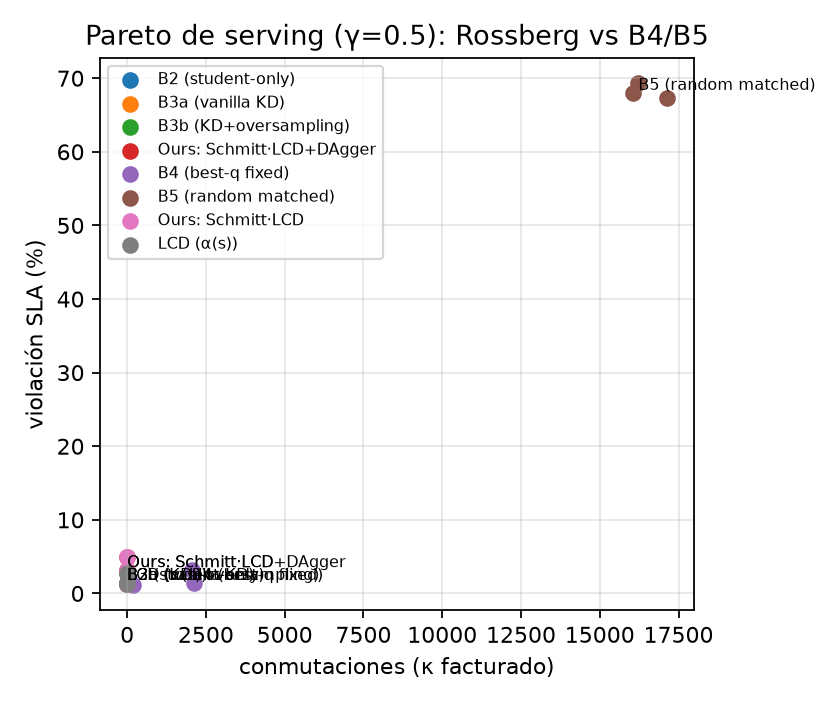
\includegraphics[width=0.72\linewidth]{fig2_pareto.png}
\caption{Serving Pareto at $\gamma{=}0.5$: transitions vs SLA
violation. Schmitt (4--6 transitions) dominates the transition axis
against B4-fixed (hundreds at comparable violation) and B5-random
(${\sim}16$k, off-scale).}
\label{fig:pareto}
\end{figure}

\paragraph{Router equalization (pre-registered sweep).} The sealed
Schmitt point matches B4-best-q at $\gamma{=}0$ ($+0.30$\,pts),
$\gamma{=}0.25$ ($+0.09$), $\gamma{=}1$ ($+0.05$); at $\gamma{=}0.5$ the
sealed point is 1.2 pts beyond the $\pm$1\,pt band, and the
pre-registered $q_{\mathrm{on}}$ sweep resolves it at
$q_{\mathrm{on}}{=}0.85$ (sealed $-0.15$\,pts, within band). Transitions:
4--6 vs.\ 200--2044 (median B4) at equalized violation —
$0.2$--$3\%$ of the B4 budget (criterion $\le 1/3$). Degenerate sweep
points without a live deadband ($q_{\mathrm{off}}=0$; effectively
always-student, coverage $1.0$) are excluded by the declared selection
rule; the full curve is reported
(\texttt{results/router\_sweep/}).
\paragraph{Transient validation (Prop 2).} Measured level sets (9 cells,
windows $\pm2$\,s around each of the 4
switches, hierarchical bootstrap; Figure~\ref{fig:transient}): narrow
heads show a detectable post-switch upward jump in $39\%$ of windows
(non-overlapping 99\% CIs, $n\ge200$), with $|\Delta \sece| \le 0.5$
pts at $\gamma=0$, $\le 0.96$ pts at $\gamma{=}0.5$; the $\gamma{=}1$
gate windows spike because the head is degenerate there. The ordinal
head concentrates the \emph{on-policy} degradation: in the short
post-burst drain windows ($n\!\approx\!500$) corn smoothECE reaches
$5.8$--$17.8\%$ vs a $1$--$2\%$ stationary level, \emph{even though}
the same deployed student's glass-box corn calibration is $\le 1.2\%$
(absolute levels of 5.8--17.8\% appear on both sides of a switch; the
drain state is where the served student is exposed). Replay-side
calibration is therefore \emph{not} deployed calibration — the central
justification of the on-policy contract, and the phenomenon the bound
of Proposition~\ref{prop:swap} is designed to absorb (its
switch-constant $C_{\mathrm{switch}}$).

\begin{figure*}[t]
\centering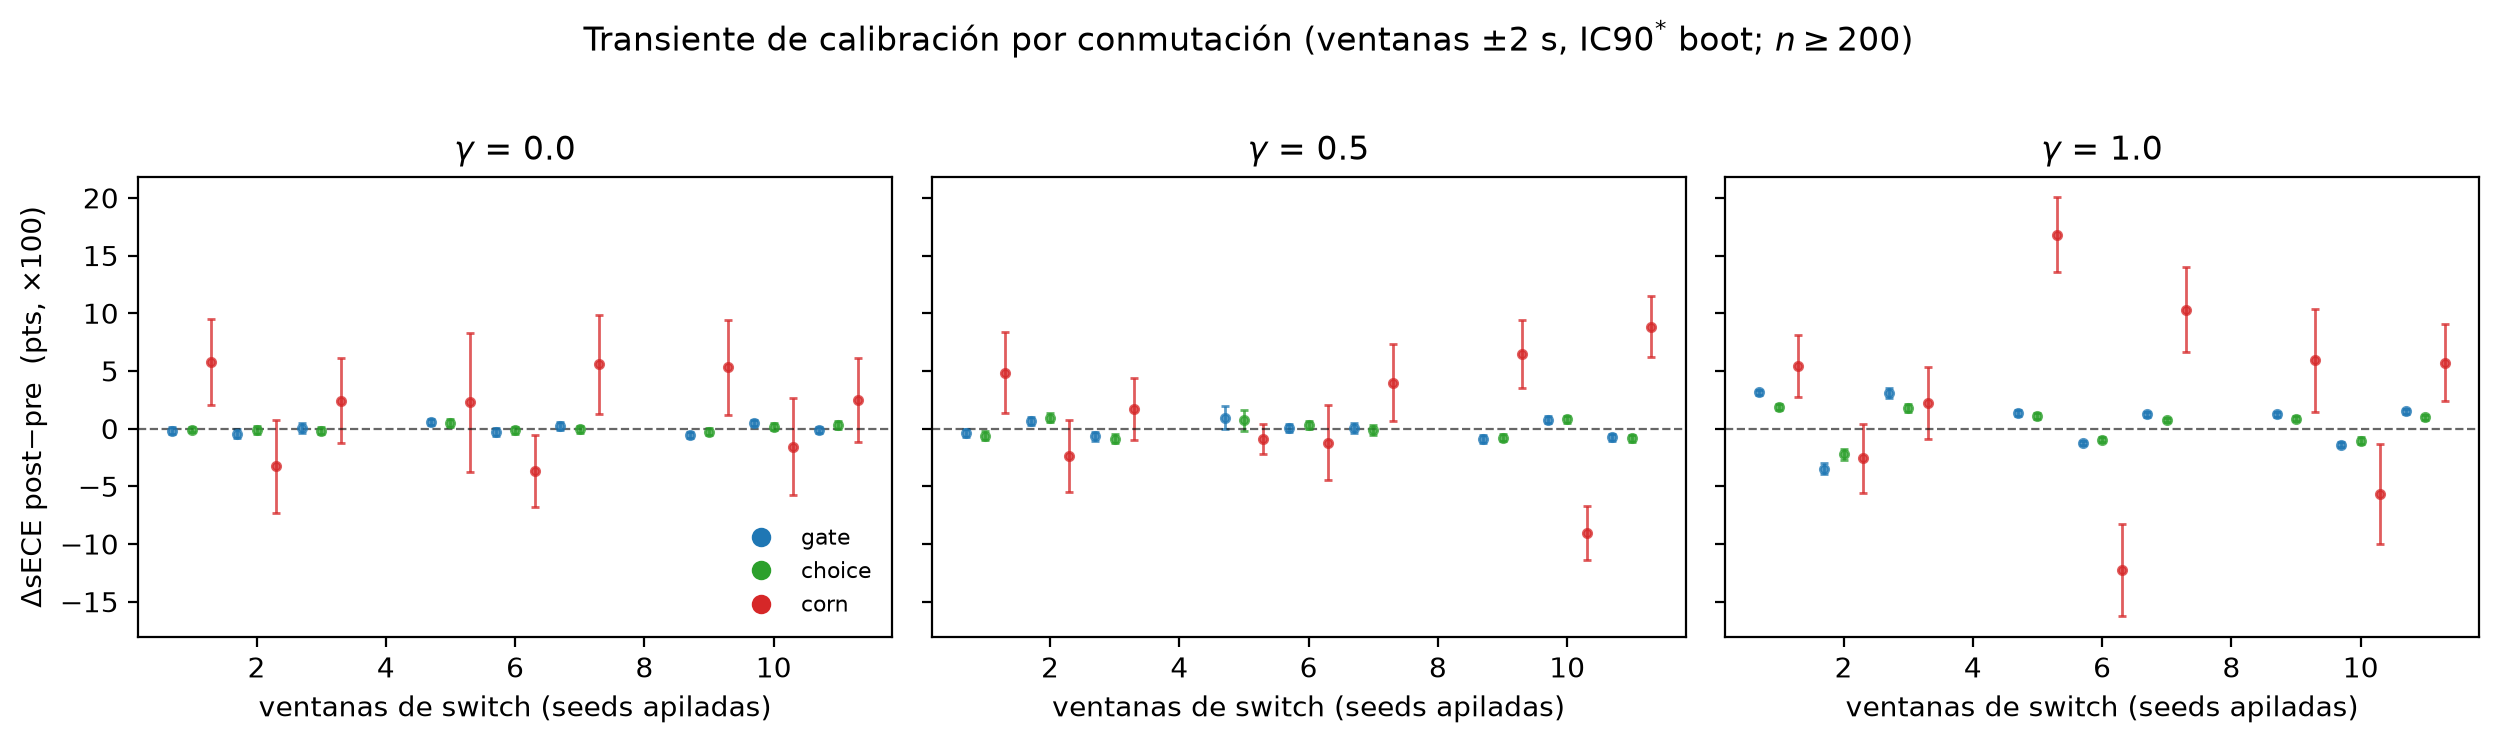
\includegraphics[width=0.92\textwidth]{fig4_transient.png}
\caption{Transient deltas per window (\emph{post}$-$\emph{pre} smoothECE,
pts): corn (red) is volatile and frequently out-of-band in the short
drain windows while gate/choice stay within $\sim$1 point; each panel
stacks the 3 seeds $\times$ 4 switch windows.}
\label{fig:transient}
\end{figure*}

\section{Honest Scorecard / Limitations}
\label{sec:limits}
\paragraph{Against the pre-registered criteria.}
(i) \emph{Adoption of smoothECE-fit temperatures} (amendment 2): adopted;
gate/choice reach $1.3$--$1.5\%$ on the $\le1\%$ goal while corn is
$\le1.2\%$ — the residual is a structural floor of the architecture
(epochs 8$\to$14 flat), documented as a capacity precondition; all
relative criteria anchor to the teacher.
(ii) \emph{LCD vs.\ B3a ($\ge$30\% hot reduction)}: NOT met on
gate/choice (insensitive, $\pm$0--3\%); met in direction (not in
magnitude) on corn: 4.7--9.3\% favorable in all $\gamma$, sign-consistent
in all seeds. Against blind oversampling (B3b): corn 36--82\% and heads
8--13\% — the blind remedy is the failure mode, and ablations attribute
the protection solely to the $\alpha(s)$ dial.
(iii) \emph{TOST at $\gamma{=}0$}: pass on gate/choice ($|\bar d| \le
0.01$ pts); corn fails only in the favorable direction ($\bar d$ up to
$-0.19$, LCD better in 3/3 seeds).
(iv) \emph{Router}: pass at all $\gamma$ (median $|\Delta$viol$| \le
0.3$\,pts; $4$--6 vs 200--2044 switches).
(v) \emph{Prop-2 transient}: measured and central to the paper (drain
windows show the on-policy effect); the pre-registered RHS formalism is
reported in the appendix.
(vi) \emph{Capacity precondition}: $\rho$ declared before the campaign;
no post-hoc re-anchoring (amendments recorded before the full grid).

\begin{table*}[t]
\centering\footnotesize
\begin{tabular}{p{5.2cm}p{5.4cm}p{5.0cm}}
\toprule
Criterion (§5) & Evidence & Status \\
\midrule
T1 smoothECE-fit adoption (amend.\ 2) & gate/choice 1.3--1.5\% vs target 1\%; corn $\le$1.2\% & adopted; structural G1 gap documented \\
T2a LCD vs B3a ($\ge$30\% hot) & +4.7--9.3\% corn $\gg$ heads $\pm$0--3\% & NO target on heads; sign consistent (3/3 seeds) \\
T2a' LCD vs B3b (blind) & corn 36--82\%; heads 8--13\% & CONFIRMED (B3b catastrophic on corn) \\
T2b TOST $\gamma{=}0$ ($\pm$0.3 pts) & gate/choice PASS; corn favorable-fail & PASS heads; corn better than B3a (3/3) \\
T3 router ($\le$1/3 B4, violation equalized) & 4--6 vs 200--2044 sw; $|\Delta$viol$|\!\le$0.3 pts & PASS all $\gamma$ (sweep $q_{\mathrm{on}}$) \\
T4 transient (Prop\ 2) & corn drain 5.8--17.8\% vs $\le$1.2\% stationary & measured; formal RHS in appendix \\
T5 capacity precondition ($\rho$) & anchored pre-campaign, no re-tuning & PASS (Amendments 1--3 pre-registered) \\
\bottomrule
\end{tabular}

\caption{Scorecard against the pre-registered success criteria
(\texttt{PRE-REGISTRATION.md} §5). Failed criteria are reported as
honest negatives with their direction; no criterion was re-defined
after seeing the full grid.}
\label{tab:scorecard}
\end{table*}
\paragraph{Known limitations.} $\gamma{=}1$ degenerates the gate head
(every event is an attack; gate tables exclude it); the ``hot'' stratum
is structurally empty in student-only deploys (served-state semantics —
the paper's point, not a bug); synthetic coupled streams, one hardware
platform; $\delt(s)$ machinery beyond the windowed measurements is
appendix-level.

\bibliographystyle{ACM-Reference-Format}
\bibliography{refs}

\appendix
\section{Formal Statements (Theory)}
\label{app:theory}
Full formal statements with hypotheses, proof sketches and the register of
hypotheses declared new vs.\ the pre-registration (E5-H1 monotone drain,
P6-H3 drain condition, P2 mixture sub-additivity) are shipped as
\texttt{theory\_props.md} in the code release.
\section{Pre-registration and Amendments}
\label{app:prereg}
The full pre-registration (\texttt{PRE-REGISTRATION.md}, sealed before
the pilot) specifies: the $\gamma$-set $\{0,0.25,0.5,1.0\}$; the sealed
operating point ($\rho_t(\mathrm{burst})=1.083$, $\rho_s=0.941$,
$L_{\max}=1.5$\,ms p99, duty $0.25$, period 8\,s); window width
$w{=}\pm2$\,s and $n_{\min}{=}200$; kernel bandwidth
$\kappa{=}0.05$; the RHS template of the bound; the expected
$\delt(s)$ reduction method; the equalization grid and fallback rule;
the two pre-registered primaries with Holm correction; the
density-ratio threshold; and the seeds
$\{(\mathrm{train},s),(\mathrm{val},100{+}s),(\mathrm{test},200{+}s),(\mathrm{rollout},300{+}s)\}$.
Amendments are recorded in the sealed appendix with evidence, not as
silent re-definitions: \emph{(A1)} the operating point was rescaled to a
physically consistent service rate (service scale $2.5\to1.0$, rates
$\times 2.5$) preserving $\rho_t,\rho_s$ and the derived deadband
exactly; \emph{(A2)} temperatures may be re-fit on the contract criterion
itself (smoothECE argmin), adopted after test-confirmation; \emph{(A3)}
the DES service clock is drawn from the hardware microbench table
(lognormal, per-deploy seeded, CV measured) with the real forward
executed only for predictions, making $\rho$ reproducible.
\section{Reproducibility}
Full one-click path: \code{make report} (tables + Figs 1--3,
\code{scripts/make_report.py});
paper tables regenerate with \code{scripts/tables_paper.py} and
Fig.~4 with \code{scripts/fig_transient.py}.
Seeds are fixed; the DES service clock samples the microbench table
with a per-deploy seed (amendment A3), verifying that the campaign
dispatch order is irrelevant to any deploy's metrics;
nets are saved per cell (\code{results/campaign/nets/}) and the
transient tooling re-deploys from those nets, reproducing every
Schmitt row exactly (9/9 cells).

\end{document}
